\chapter{Omringende logica}
\label{periphery}

Een heleboel logische blokken, zoals decoders, drivers, pass-gates en buffers zitten verwerkt in de geheugenstructuur.
In dit hoofdstuk worden deze componenten van wat dichterbij onderzocht.

\section{Decoders}
Een decoder is een logische blok dat een uitgang selecteert op basis van een geëncodeerde bus van ingangen: uit een combinatie van N ingangen, gaat er steeds één van $2^N$ uitgangen actief hoog worden\footnote{Er is nog een enable-controlesignaal, wanneer dit actief laag is, gaan alle uitgangen actief laag zijn.}. Aangezien het aantal global blocks, woordlijnen en bitlijnen nog niet vastgelegd werd, werd er een gamma aan decoders ontworpen gaande van een 2-naar-4 decoder tot en met een 9-naar-512 decoder. Grotere decoders worden opgebouwd uit kleinere decoders. Dit kan gedaan worden op 2 manieren; volgens een tree patroon (\ref{fig:decoder1}) of volgens een grid patroon (\ref{fig:decoder2}). In de volgende secties wordt het ontwerp van beide manieren toegelicht en vergeleken.

\begin{figure}[!ht]
\centering
\subfloat[Decoder type 1]{ 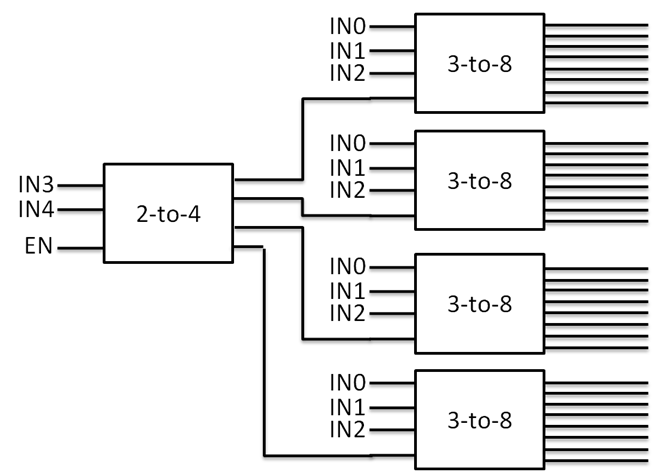
\includegraphics[width=0.45\textwidth] {../fig/hfdst-decoders-type1.png} \label{fig:decoder1}}
\subfloat[Decoder type 2]{ 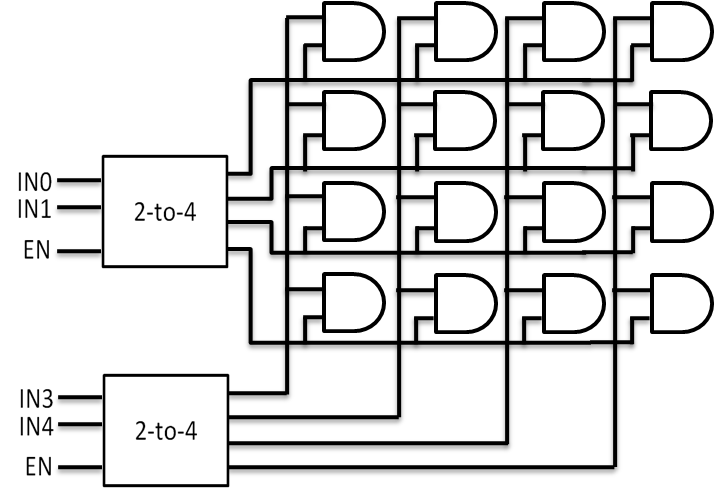
\includegraphics[width=0.45\textwidth] {../fig/hfdst-decoders-type2.png} \label{fig:decoder2}}
\caption{Opbouw voor grotere decoders}\label{fig:basisdecoders}
\end{figure}

\subsection{De tree decoder}
De tree decoder is een decoder met een meerlaagse structuur dat zich uitwaaiert naar de uitgangen. De basisblokken van deze decoder zijn een 2-naar-4 decoder (figuur \ref{fig:decoder2to4}) en een 3-naar-8 decoder (figuur \ref{fig:decoder3to8}). Het principe van de tree decoder is als volgt: met x-naar-$2^x$ en y-naar-$2^y$ decoders kan men een $x+y$-naar-$2^{x+y}$ realiseren door ze te cascaderen. De MSBs worden aangesloten aan de eerste laag. Dit wordt geïllustreerd in de vorm van een 5-naar-32 decoder in figuur \ref{fig:decoder1}. 
\begin{figure}[!ht]
\centering
\subfloat[2 naar 4 decoder]{ 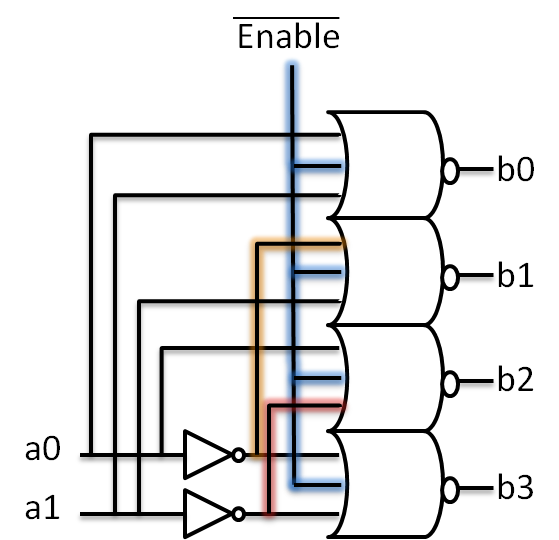
\includegraphics[width=0.5\textwidth] {../fig/hfdst-decoders-2to4.png} \label{fig:decoder2to4}}
\subfloat[3 naar 8 decoder]{ 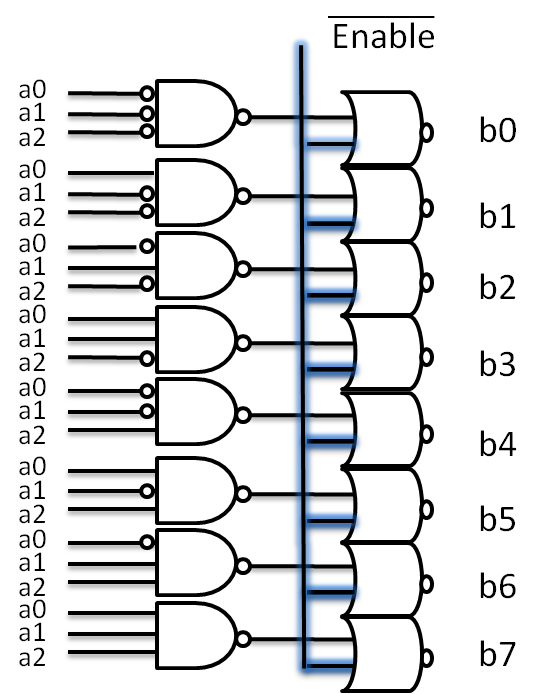
\includegraphics[width=0.5\textwidth] {../fig/hfdst-decoders-3to8.png} \label{fig:decoder3to8}}
\caption{basis decoders}
\end{figure}

\subsection{De grid decoder}
De grid decoder heeft een tweelaagse structuur. De eerste laag bestaat uit een aantal 2-naar-4 en/of 3-naar-8 decoders die in parallel staan. De verschillende uitgangen van deze eerste laag worden dan met AND-gates samen gevoegd in een tweede laag. Om glitches te voorkomen is het belangrijk dat al de signalen gelijktijdig binnen komen in de AND-gates, daarom werd de topologie van de 2-naar-4 decoder van figure \ref{fig:decoder2to4} veranderd tot een NAND-NOR topologie zoals die van de 3-naar-8 decoder in figuur \ref{fig:decoder3to8}. Bij grotere decoders worden de uitgangen van de eerste laag aangesloten aan groot aantal AND-gates. Omwille van deze grote fan-out moeten de uitgangen van de eerste laag gebufferd worden met overeenkomstig geschaalde inverters. Omdat er dus toch al minstens 2 inverters voor de AND-gates worden geplaatst, worden deze geïmplementeerd als NOT-gate + NOR-poort i.p.v. NAND-poort + NOT-poort. Tabel \ref{tab:griddecoder} geeft de hoeveelheid basisdecoders weer in de eerste laag van de grid decoder en het aantal AND-gates de tweede laag, in functie van het aantal inputs.

\begin{table}
\begin{center}
\begin{tabular}{llll}
\hline
\# inputs decoder & \# 2-naar-4 decoders & \# 3-naar-8 decoders & \# AND-gates\\
\hline
4 & 2 & 0 & 16\\
5 & 1 & 1 & 32\\
6 & 0 & 2 & 64\\
7 & 2 & 1 & 128\\
8 & 1 & 2 & 256\\
9 & 0 & 3 & 512\\
\hline
\end{tabular}
\end{center}
\caption{Aantal gates in de grid decoder}
\label{tab:griddecoder}
\end{table}

\subsection{Vergelijkende studie}
Eens ontworpen, kunnen de tree en grid decoders met elkaar vergeleken worden. Naast de gebruikelijke oppervlakte, energie en delay worden ook glitches, mismatch en delay tussen verschillende addressen onderzocht. \\
Zoals in figuur \ref{fig:decoder_a} gezien kan worden, schaalt de oppervlakte van de grid decoder veel minder dan die van de tree decoder bij een groot aantal ingangen. De plotse stijging in de oppervlakte van de tree decoder met 8 ingangen kan verklaar worden door het gebruik van een extra laag in de boomstructuur. \\
Het energieverbruik wordt vergeleken in figuur \ref{fig:decoder_ed}. De grid decoder verbruikt minder energie in functie van het aantal ingangen. Sommige signalen in de tree decoder zullen diep doorrimpelen, waardoor er meer gates zullen schakelen dan in de grid decoder.  Het overbodig schakelgedrag van de tree decoder zou tot zekere mate ingeperkt kunnen worden door de topologie van de basisdecoders (figuur \ref{fig:basisdecoders}) te wijzigen zodat de enable vooraan komt te staan.\\
De delay van de decoders kan ook afgelezen worden in figuur \ref{fig:decoder_ed}. Beide types decoders hebben ongeveer dezelfde delay. Bij grotere grid decoders kan de extra delay verklaard worden door de extra latency van de buffers.\\
Verder werden glitches onderzocht. In beide decoders is er de mogelijkheid dat er glitches opduiken. Het probleem bij deze decoders is het gebuik van de NOR-gates. Wanneer de twee ingangs-signalen van de NOR-gate niet gelijktijdig toekomen (zie figuur \ref{fig:decoder_glitch}), kan de uitgang van de gate tijdelijk actief hoog getrokken worden, om vervolgens weer laag getrokken te worden. Bij de tree decoder is het nagenoeg onmogelijk om deze ongelijktijdigheid te overkomen: sommige signalen moeten immers meer lagen doorlopen dan andere vooraleer de NOR-ingang bereikt wordt. Bij de grid decoder daarentegen kan een glitch opduiken als de buffers die de tweede laag aansturen een asymetische delay hebben. Dit kan bijvoorbeeld voorkomen bij een 5-naar-32 decoder. De uitgangen van de 2-naar-4 decoder en de 3-naar 8-decoder in deze decoder hebben een andere last. Sommige buffers kunnen echter suboptimaal ontworpen worden zodat de NOR-ingangssignalen alsnog gelijktijdig toekomen.\\
Na een snelle mismatch-analyse blijkt dat de grid decoder minder variatie toont in dynamisch energieverbruik en delay dan de tree decoder. Tenslotte heeft de tree decoder een grotere spreiding wat delay betreft, afhankelijk van het vorige en huidige addres: wanneer er slechts één adresbit schakelt, kan het voorkomen dat dit signaal slechts kort moet doorrimpelen tot de uitgang. Dit ziet men minder in de grid decoder. \\
Na het vergelijken van beide decoders wat oppervlakte, energie, delay, glitches, mismatch en delay betreft, komt de grid decoder er als beste uit en zal deze dan ook gebruikt worden in het finale ontwerp.


\begin{figure}[!ht]
\centering
\subfloat[Oppervlakte]{ 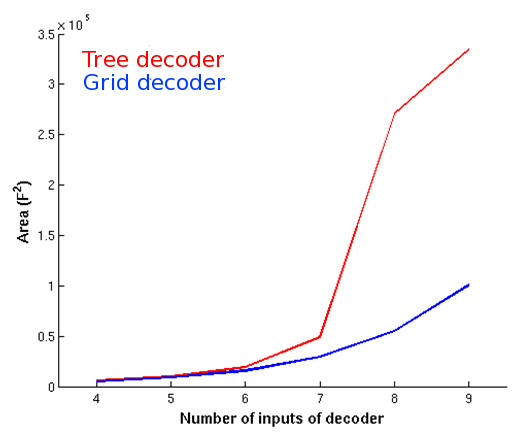
\includegraphics[width=0.5\textwidth] {../fig/hfdst-decoders-a.png} \label{fig:decoder_a}}
\subfloat[Energie en delay]{ 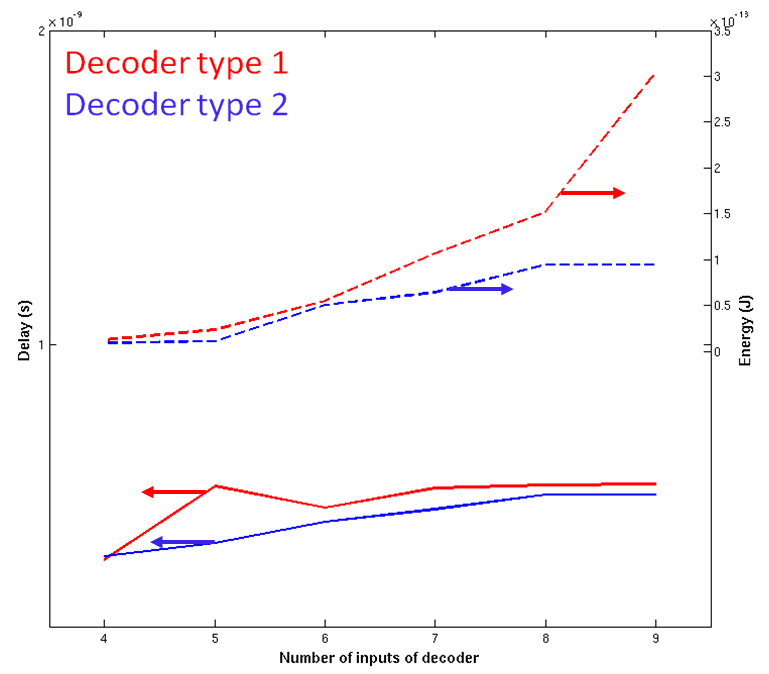
\includegraphics[width=0.5\textwidth] {../fig/hfdst-decoders-ed.png} \label{fig:decoder_ed}}
\caption{Vergelijking van decoder types}
\end{figure}


%\begin{figure}[!ht]
%  \centering
%  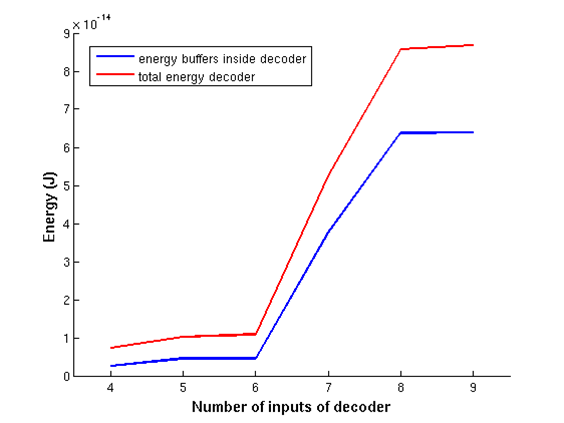
\includegraphics[width=0.8\textwidth]{../fig/hfdst-decoders-egrid.png}
%  \caption{Energie verbruik in griddecoder}
%  \label{fig:decoder_egrid}
%\end{figure}

\begin{figure}[!ht]
  \centering
  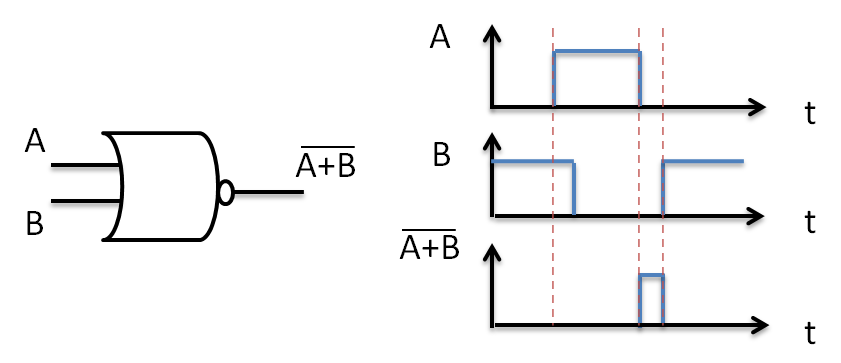
\includegraphics[width=0.8\textwidth]{../fig/hfdst-decoders-glitch.png}
  \caption{Glitch in NOR-gate}
  \label{fig:decoder_glitch}
\end{figure}


\section{Buffers}
Kleine CMOS gates kunnen slechts een beperkte hoeveelheid stroom leveren. Wanneer de uitgang van deze gates aangesloten wordt op een grote capacitieve last, duurt het lang voordat deze last is op- of ontladen. Soms is het niet aangewezen om deze gate zelf op te schalen, hierdoor neemt de intrinsieke last immers toe en gaan de gates van de vorige trap mogelijk niet meer genoeg stroom kunnen leveren om de ingang van de gate snel te sturen. In dit geval is het aangewezen om de uitgang van de gate te bufferen. Een ideale buffer heeft geen ingangscapaciteit en kan oneindig veel stroom leveren om eender welke last onmiddelijk te sturen. In de praktijk worden buffers geïmplementeerd door een even aantal invertoren te cascaderen. De eerste inverter in de ketting is klein genoeg zodat de gebufferde gate hier geen last van ondervindt, de volgende inverters in de ketting worden systematisch opgeschaald zodat de laatste inverter in de ketting voldoende stroom kan leveren om de last te sturen. 
Buffers worden op drie plaatsen in de geheugen architectuur gebruikt. Ten eerste om de woordlijnen aan te sturen. Ten tweede om de referentielogica aan te sturen en tenslotte  tussen de eerste en tweede laag in de grid decoders. Tabel \ref{tab:buffer} geeft een overzicht van de oorsprong van de last en de waarde van de last die de verschillende buffers moeten aansturen.\\
De buffers werden ontworpen met de methode van logical effort waarbij het aantal stages en de sizing van elke stage werd bepaald volgens het volgende stappenplan:
\begin{enumerate}
\item Bepaal de path effort $F = GH$ waarbij $G = 1$ aangezien we enkel met inverters werken en $H = \frac{C_{out}}{C_{in}}$
\item Het aantal stages wordt bepaald door $\hat{N} = log_{4}F$. Hierbij werd er voor een stage effort van 4 gekozen voor een optimale delay\cite{Sutherland:1999:LED:298513}. \^{N} wordt dan afgerond tot een even getal N voor de woordlijn- en referentiebuffers en tot een oneven getal voor de decoderbuffers.
\item N wordt dan gebruikt om een nieuwe stage effort \^{f} te berekenen met de formule $\hat{f} = F^{1/N}$.
\item Tenslotte kunnen de de groottes van de verschillende invertoren in de chain berekend worden met de nieuwe stage effort $\hat{f} = gh$.
\end{enumerate}
Figuur \ref{fig:refbuffer} illusteert de ongebufferde en gebufferde signalen die naar de referentielogica gaan, voor verschillende groottes van last.

\begin{table}
\begin{center}
\begin{tabular}{ccc}
\hline
 & Type Last & \# Capaciteit\\
\hline
Woordlijnbuffer & 1 Transistorgate &  $\#BL*0,18fF$\\
Referentiebuffer & 1 Nor + 1 Inv &  $\#BL*0,93fF$\\
Decoderbuffer & 1 Nor & (4-64)$*0.58fF$\\
\hline
\end{tabular}
\end{center}
\caption{Lasten in de verschillende buffers}
\label{tab:buffer}
\end{table}

\begin{figure}[!ht]
  \centering
  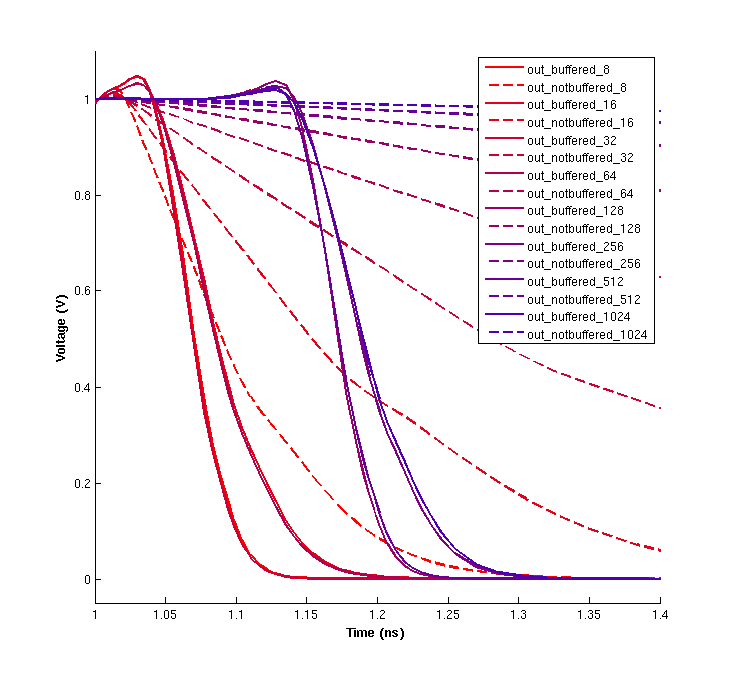
\includegraphics[width=0.8\textwidth]{../fig/hfdst-buffers-refbuffer.png}
  \caption{Gebufferde en ongebufferde signalen naar de referentie logica}
  \label{fig:refbuffer}
\end{figure}

\section{BL- en WL-drivers}
Elk global block heeft ingangslijnen voor geëncodeerde BL- en WL-signalen. Het zou energieverspilling zijn om deze signalen naar alle GB te laten propageren, terwijl er slechts 1 GB in werking zal treden omdat het bijhorende $GB\_{Enable}$-controlesignaal actief hoog is. Deze vertakte lijnen, die over heel de chip lopen zouden immers een aanzienlijke capacitieve last bevatten (zie figuur \ref{fig:nodrivers}). Het is beter om deze BL- en WL-signalen tussenin nog laten gebufferd worden zoals op figuur \ref{fig:drivers}. Deze drivers kunnen eenvoudig gerealiseerd worden met AND-gates in een NAND-gate + NOT-gate implementatie.
De energiewinst hangt natuurlijk samen met de onwerpparameters NoGB, NoBLpLB en NoWLpB: er zijn NoGB $GB\_{Enable}$ signalen, die elk $\log_2 NoBLpLB +\log_2 NoWLpB$ drivers moeten aansturen. Deze extra benodigde energie moet natuurlijk kleiner zijn dan de energie die wordt gewonnen door een groot deel capaciteit van de lijnen te vermijden. Om exact deze cijfers te weten is een parasitaire layout extraction nodig, wat in dit werk niet is uitgevoerd.

\begin{figure}[h!]
  \centering
  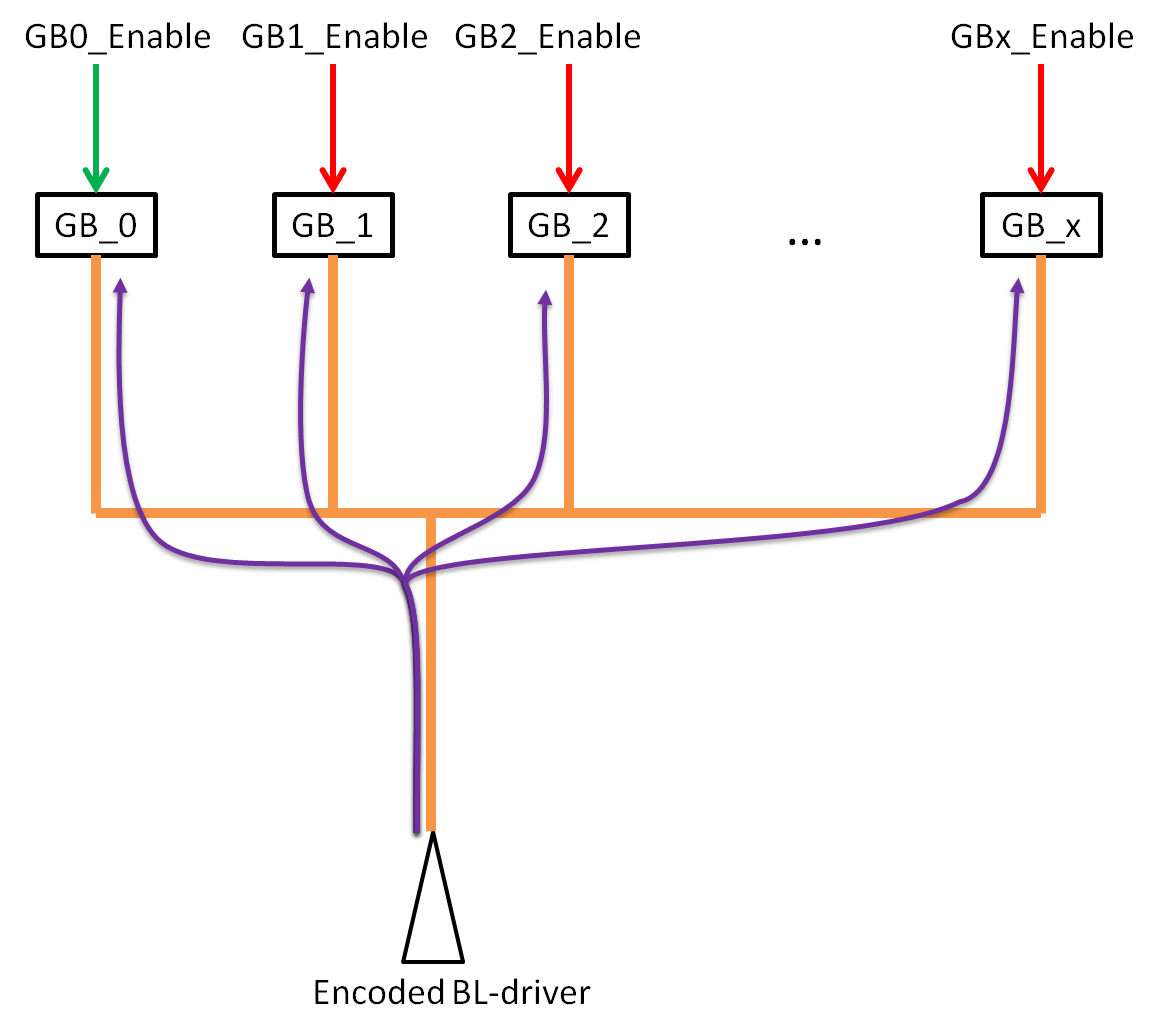
\includegraphics[width=0.5\textwidth]{../fig/hfdstk-periphery-nodrivers.png}
  \caption{Off-chip driver moet enorme last opladen}
  \label{fig:nodrivers}
\end{figure}
\begin{figure}[h!]
  \centering
  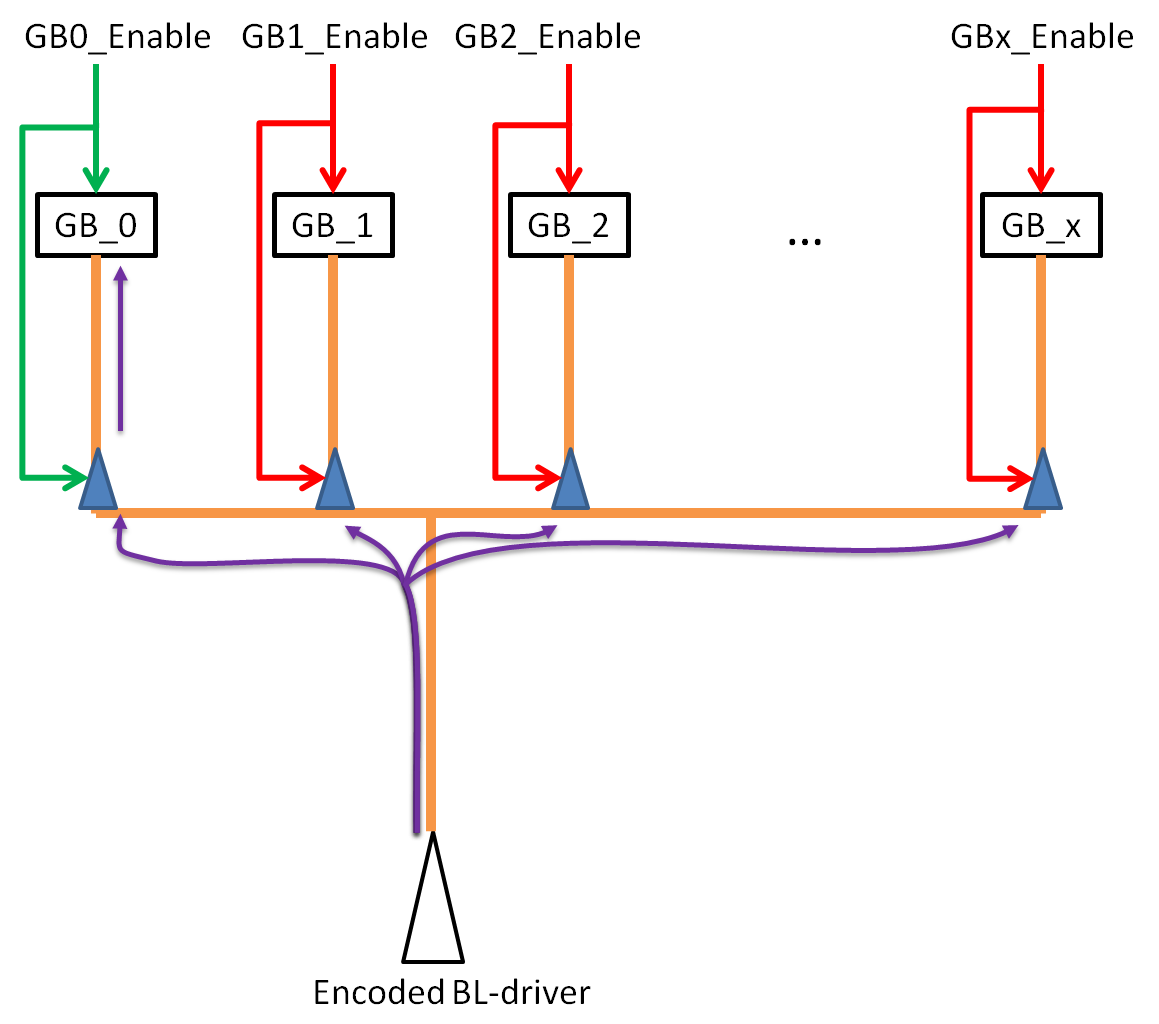
\includegraphics[width=0.5\textwidth]{../fig/hfdstk-periphery-drivers.png}
  \caption{Tussenin wordt gebufferd, zodat niet hele lijnen moeten worden opgeladen}
  \label{fig:drivers}
\end{figure}

\section{Passgates}
Passgates zijn schakelaars die de spanning van een laagimpedant knooppunt doorlaten naar een hoogimpedant knooppunt. Idealiter heeft de passgate geen weerstand wanneer hij aanstaat. In de praktijk zal er altijd een beetje weerstand zijn, dit heeft als gevolg dat er een kleine RC-delay vooraleer het hoogimpedante punt is geladen/ontladen tot de waarde van het laagimpedante punt.
Een passgate kan gerealiseerd worden met een nMOS transistor, een pMOS of een combinatie van beiden.
In wat volgt worden de verschillende scenario's besproken die kunnen optreden wanneer de schakelaar aangezet wordt, de passgate zal immers niet altijd stroom kunnen leveren om het hoogimpedante knooppunt te (ont)laden.

\subsection{nMOS passgate}
De opstelling is het circuit van figuur \ref{fig:passgate1}. Afhankelijk van de (initiële) waardes van Vx en Vs, kunnen volgende situaties optreden.

\begin{figure}[h!]
  \centering
  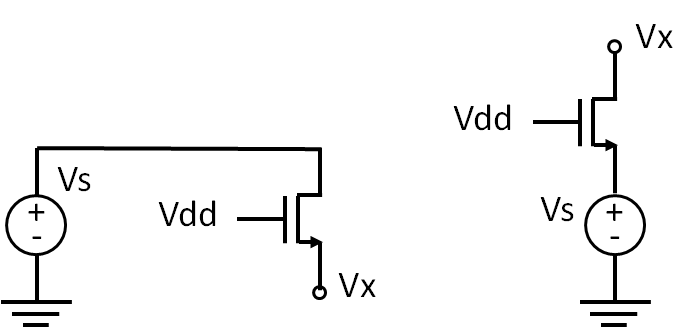
\includegraphics[width=0.5\textwidth]{../fig/hfdst-periphery-passgate1.png}
  \caption{nMOS passgate opstelling. a: Vs > Vx, b: Vs < Vx}
  \label{fig:passgate1}
\end{figure}

\begin{itemize}
\item Vx > Vs en Vdd - Vs > Vtn: de transistor gaat Vx ontladen tot Vs.
\item Vx > Vs en Vdd - Vs < Vtn: de transistor staat af, er gebeurt niets.
\item Vx < Vs en Vs < Vdd - Vtn: de transistor levert stroom tot Vx is opgeladen tot Vs.
\item Vx < Vs, Vs > Vdd - Vtn en Vx < Vdd - Vtn: de transistor gaat Vx opladen tot Vdd - Vtn.
\item Vx < Vs, Vs > Vdd - Vtn en Vx > Vdd - Vtn: de transistor staat af, er gebeurt niets.
\end{itemize}

\subsection{pMOS passgate}
De opstelling is het circuit van figuur \ref{fig:passgate2}. Er kunnen wederom verschillende situaties optreden.

\begin{figure}[h!]
  \centering
  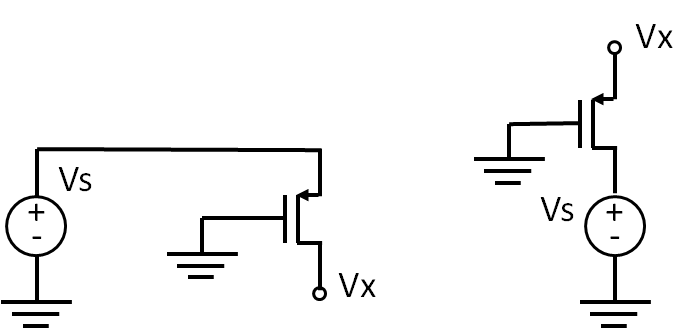
\includegraphics[width=0.5\textwidth]{../fig/hfdst-periphery-passgate2.png}
  \caption{pMOS passgate opstelling. a: Vs > Vx, b: Vs < Vx}
  \label{fig:passgate2}
\end{figure}

\begin{itemize}
\item Vs > Vx en Vs > |Vtp|: de transistor gaat Vx opladen tot Vs.
\item Vs > Vx en Vs < |Vtp|: de transistor staat af, er gebeurt niets.
\item Vs < Vx en Vs > |Vtp|: de transistor levert stroom tot Vx is ontladen tot Vs.
\item Vs < Vx, Vs < |Vtn| en Vx > |Vtp|: de transistor gaat Vx ontladen tot |Vtp|.
\item Vs < Vx, Vs < |Vtn| en Vx < |Vtn|: de transistor staat af, er gebeurt niets.
\end{itemize}

Er zijn dus spanningszones waarvoor de passgate niet functioneert, het is belangrijk te weten wat deze zones zijn, zodat het circuit ontworpen wordt om deze zones te vermijden. 
Op figuur \ref{fig:passgate3} worden deze zones in kaart gebracht voor een nMOS, een pMOS en een complementaire passgate, zowel voor LVT als HVT transistoren. Er dient opgemerkt te worden dat de passgates niet (of slechts even) aanstaan voor sommige zones, maar dat de uiteindelijke fout nog meevalt.
Als Vs bijvoorbeeld 0,9V bedraagt voor een nMOS passgate en Vx initieel 0,85V (met Vdd 1V), gaat de transistor geen stroom leveren, maar bedraagt de uiteindelijke fout 'slechts' 50mV.
In deze fout zit nog geen ladingsinjectie inbegrepen, eenmaal de passgate afschakelt is de injectie onvermijdelijk.
Zowel de LVT als de HVT complementaire passgates vertonen geen dode zones. Voor performantieredenen is geopteerd voor de LVT transistoren in het geheugenontwerp.

\begin{figure}[!ht]
\centering
\subfloat[CLVT]{ 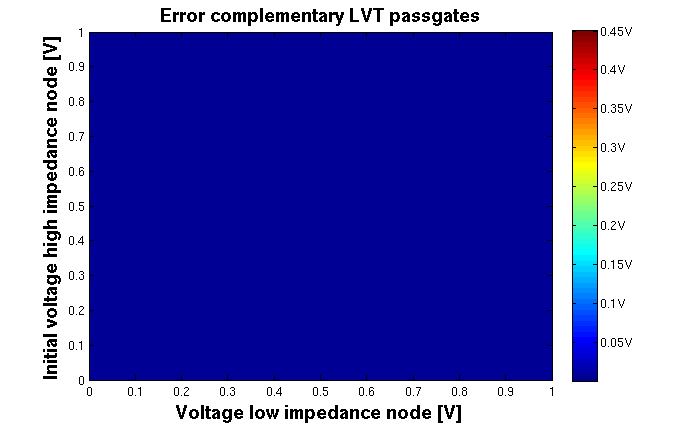
\includegraphics[width=0.5\textwidth] {../fig/hfdstk-periphery-CLVT.png}}
\subfloat[CHVT]{ 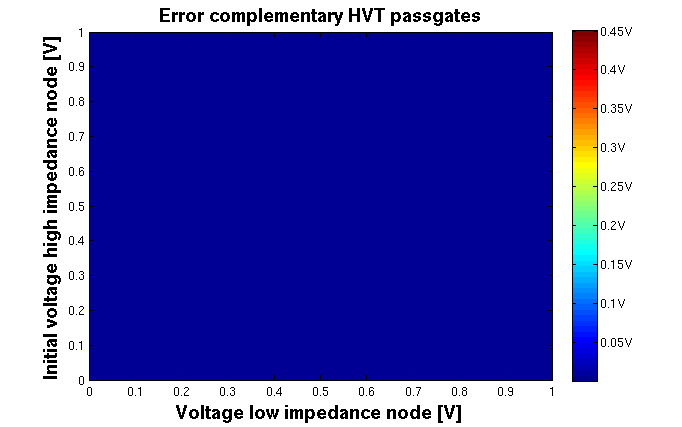
\includegraphics[width=0.5\textwidth] {../fig/hfdstk-periphery-CHVT.png}}\\
\subfloat[NLVT]{ 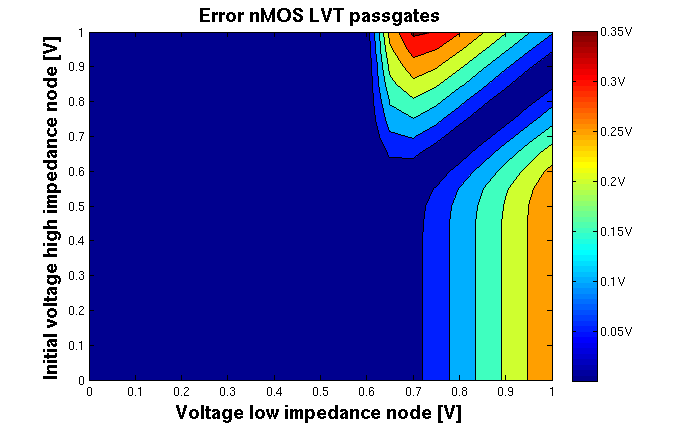
\includegraphics[width=0.5\textwidth] {../fig/hfdstk-periphery-NLVT.png}}
\subfloat[NHVT]{ 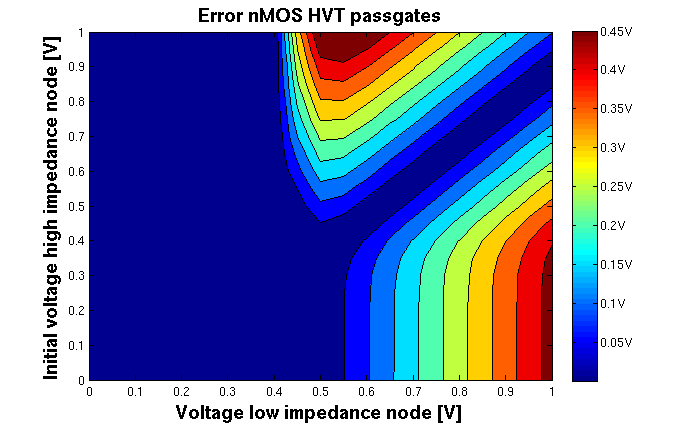
\includegraphics[width=0.5\textwidth] {../fig/hfdstk-periphery-NHVT.png}}\\
\subfloat[PLVT]{ 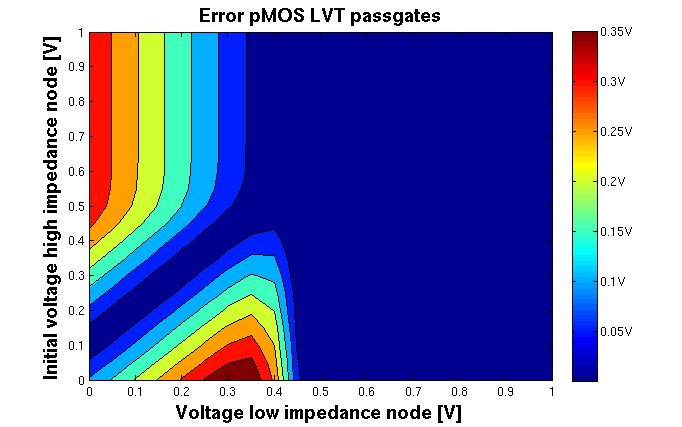
\includegraphics[width=0.5\textwidth] {../fig/hfdstk-periphery-PLVT.png}}
\subfloat[PHVT]{ 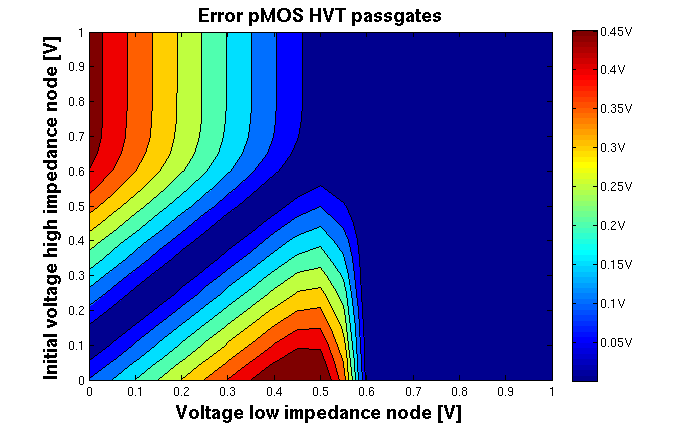
\includegraphics[width=0.5\textwidth] {../fig/hfdstk-periphery-PHVT.png}}
\caption{Dode zones voor verschillende types passgates}
\label{fig:passgate3}
\end{figure}



\section{Besluit}
Bij het ontwerpen van een geheugen is er nood aan een aantal klassieke bouwblokken: decoder, buffers, passgates. Ontwerpproblemen en -keuzes werden overlopen en toegelicht. Bij de decoders werd er gekozen voor een grid architectuur om glitches te vermijden. Buffers werden ontworpen met logical effort, waarbij het aantal stages werd bepaald in functie van de last. En tenslotte bleek uit de analyse van de pass-gates dat er nood was aan complementaire pass-gates met lage Vt.
